GoTxn is a transaction system we implemented and verified with the goal of
making crash safety and concurrency simple for a storage system implemented on
top. Transactions appear to run atomically both on crash and to other threads.
The GoTxn specification formalizes this property, which we use in DaisyNFS to
enable sequential reasoning for a concurrent file system (described in
\cref{ch:daisy-nfs}).

This chapter describes GoTxn's implementation, top-level specification, and
several aspects of the proof. The implementation is composed of a software stack
with several layers; each layer implements a new interface on top of one
below. The proof follows the same structure, with several new specifications for
intermediate layers. Of particular note are the
transaction-refinement specification for the transaction system, the lifting
specification for the journaling layer, and the abstraction for the write-ahead
log layer.

While as part of this thesis we only used GoTxn to implement and verify a file
system, the system and its specification are generic for any
storage system implemented on top, as long as its operations are implemented
using transactions.

GoTxn faces three key challenges in its specification, design, and proof.
First, GoTxn's specification is stated in terms of programs using the
transaction system, and not all programs will observe atomic transactions ---
for example, accessing global variables or the network in the middle of a
transaction is not atomic. To state a provable specification for GoTxn we needed
a formalization of \emph{safe transactions}, described in \cref{sec:txn:transaction-refinement},
which obey some restrictions that the specification assumes the caller follows.

The second challenge is supporting an in-memory allocator, which is necessary
for the file system to get good performance but appears to violate GoTxn's rule
that transactions do not access shared memory since allocating and
freeing affect other transactions immediately, not at commit time.
To address this challenge we include an
allocator in the GoTxn API and proof. A non-deterministic,
\emph{under-specification} of the allocator makes its behavior serializable, and
\cref{ch:daisy-nfs} demonstrates that this allocator is usable by using it in
the DaisyNFS verified file system.

Finally, this specification is related to a concrete implementation, and thus
requires a proof using a program logic. The proof manages the complexity of
GoTxn's implementation by combining a \emph{lifting-based specification} that
captures the journaling layer's crash atomicity (\cref{sec:txn:lifting}) with a
simulation proof that captures how two-phase locking's concurrency control works
(\cref{sec:txn:refinement}).

\section{Programming with GoTxn}
\label{sec:txn:api}

\begin{figure}
\begin{minted}{go}
type Addr struct {
  Blkno  uint64
  Offset uint64
}

// starting and stopping a transaction
func Begin() *Txn
func (tx *Txn) Abort()
func (tx *Txn) Commit()

// operations within a transaction
func (tx *Txn) Read(a Addr, sz uint64) []byte
func (tx *Txn) ReadBit(a Addr) bool
func (tx *Txn) Write(a Addr, d []byte)
func (tx *Txn) WriteBit(a Addr, d bool)

// allocator API
func NewAllocator(max uint64) *Allocator
func (a *Allocator) Alloc() uint64
func (a *Allocator) Free(n uint64)
func (a *Allocator) MarkUsed(n uint64)
\end{minted}
  \caption[GoTxn API]{The API for the transaction system and allocator. Reads and writes
    between \cc{Begin} and \cc{Commit} appears to execute atomically on disk and
    for other threads, while \cc{Abort} guarantees the transaction has no
    effect. The allocator's \cc{Alloc} and \cc{Free} operations are safe to call
    concurrently.}
\label{fig:txn-api}
\end{figure}

The transaction system exports a transactional API for durable, on-disk objects. The caller can wrap a whole
sequence of reads and writes in a transaction between a call to \cc{Begin()} and
\cc{Commit()}, and the transaction system guarantees that all of the operations
appear to execute atomically (that is, all at once). The
programming interface is listed in \cref{fig:txn-api}. Reads and writes can be
for objects smaller than a full 4KB block, which improves concurrency.
Transactions make it much easier to implement a correct storage system by
handling the challenges of crash safety and concurrency, so that the system on
top only needs to implement its own data structures and operations on top of
disk objects.

To use GoTxn, a storage system wraps all of the code for every operation in a
single transaction in order to make it atomic. The \cc{Begin()} call creates an
empty transaction.
The body of the
transaction appears to execute atomically when the operation finishes it
with \cc{Commit}, or the transaction is discarded with no effect on
\cc{Abort}. Reads and writes operate on addresses that specify a
position by giving a block number and an offset in bits (always less
than $4096 \cdot 8$, the number of bits in a block). The \cc{Read}
method requires an explicit size argument while the size of a
\cc{Write} is implicit in the size of the \cc{data} slice. We separate
out the bit-sized operations to \cc{ReadBit} and \cc{WriteBit} (rather
than using a single-element byte slice) to simplify the specification.

\Cref{fig:txn-api} also includes an API for allocation alongside the transaction
API.\@ The allocator should be considered part of the transaction system API
insofar as its operations are allowed within a transaction. In contrast, using
other shared memory within a transaction is not permitted since it would
compromise the atomicity guarantees --- the transaction system acquires locks to
make reads and writes seem atomic, but it doesn't have any locking discipline
for other state. \Cref{sec:txn:transaction-refinement} explains these restrictions and an
\emph{under-specification} technique for fitting the
in-memory allocator API into GoTxn's atomicity guarantee.

%% The state of the transaction system (the transactional disk transactions
%% manipulate) looks much like a flat array of bytes.
%% However, the caller cannot
%% read and write arbitrary regions of this array due to restrictions in the
%% gojournal code and proof. all reads and writes must be within a single 4kb block
%% on disk, and of a power-of-two number of bytes or a single bit.

% In practice the file system uses three kinds of objects: full blocks are used
% for data (both for directories and data files), bit objects comprise the inode
% and block allocators, and 128-byte objects are used to represent inodes. The
% file-system statically allocates regions for the inodes, allocator bitmaps,
% and data blocks, so that object sizes never change.

As described in \cref{sec:txn:impl}, GoTxn is implemented using two-phase
locking. As a result, a transaction acquires a per-address lock on every address
it reads or writes along the way. Acquiring multiple locks during a transaction
creates the possibility for deadlocks, if two threads acquire locks with
different orderings, and the specification does not forbid
deadlocks.\footnote{Liveness reasoning is quite challenging when
combined with concurrency. However, it would be interesting to specify and
verify deadlock freedom, a safety property, without verifying the liveness of the
whole system.} The two-phase locking
implementation does not implement a specific lock acquisition order, leaving it
to the calling code to avoid deadlock --- for example, in DaisyNFS the
implementation of \cc{RENAME} makes sure to lock the smaller inode number first
(by reading from it) if the rename is between different directories.

\section{Specifying GoTxn using refinement}%
\label{sec:txn:spec}

At a high level, GoTxn makes transactions atomic. This chapter formalizes this
intuitive definition in the form of \emph{program refinement}. Later in
\cref{ch:daisy-nfs} we build upon this specification to show how it enables
sequential reasoning. Program refinement is defined in terms of
\emph{refinement}, which relates code to a specification. Abstractly, refinement
from a code program to a specification says that the behaviors of the code are a
subset of the behaviors of the specification.

To define the specification, we need to be more precise about what a program is
and how it executes to talk about the server loop program. We
write $p : \gooselayer{X}$ to say $p$ is a Go program written using operations
from layer X.
Layer operations are always atomic transitions in a state machine. Layers will
be one of Sys, Txn, or Disk, where Sys is a
stand-in for an arbitrary system implemented on top of GoTxn. We write this
generically to emphasize that the GoTxn specification does not fix how the
caller uses transactions; in practice it will be instantiated with the NFS state
machine for DaisyNFS.
The Txn layer consists of the GoTxn API, with reads and writes over a logical
disk and the ability to wrap these into an atomic transaction. The
Disk transition system is formalized in Coq as part of the GoTxn proof,
and assumes reads and writes of 4KB blocks are atomic. All layers
include concurrent threads that interleave layer
operations, basic heap operations on pointers, slices, and maps, and computation
on primitives like integers and structs.

The correctness for GoTxn relates a \emph{spec program} $p : \gooselayer{Txn}$
that uses transactions to its implementation. These specification programs can
invoke transactions, which we write $\atomically{\cc{f}}$ to represent a
transaction running \cc{f}, which in turn might have calls to Read and Write
from the GoTxn API. A specification program $p$ has an associated implementation
program $\mathrm{link}(\sdfy, \txncode) : \gooselayer{Disk}$, where we ``link''
with the GoTxn code. Linking has two effects: first it expands
$\atomically{\cc{f}}$ to a
sequence like \cc{tx := Begin(); f(tx); tx.Commit()} (with some additional code
handling aborts), and second it replaces calls to the Txn abstract Read and
Write operations with the GoTxn implementations at the Disk abstraction layer.

Refinement relates two programs in terms of their visible behavior, which is
used in the specification
to connect a program written at the transaction layer to its
implementation at the disk layer. This notion of refinement also incorporates
crashes into the outcomes of executing the program and gives it a corresponding specification.
For the purposes of this work, the visible
behavior is always network I/O, corresponding to receiving requests for the
system or responding to them (for example, processing NFS requests).

\begin{definition}[Refinement]
  An implementation program $p_{c}$ refines a specification program $p_{s}$,
written $p_{c} \refines p_{s}$, if whenever there are initial states
$\sigma_{s}$ and $\sigma_{c}$ satisfying $\mathrm{init}(\sigma_{s}, \sigma_{c})$
and $p_{c}$ can execute from $\sigma_{c}$ and produce a trace of network I/O
$\textit{tr}$, then $p_{s}$ can execute from $\sigma_{s}$ and produce the same trace
$\textit{tr}$.  Execution might involve crashing and restarting a program (potentially
multiple times), wiping out any in-memory state after each crash.
  \label{def:refinement}
\end{definition}

The intuition behind the notation $p_{c} \refines p_{s}$ is that the set of
behaviors of $p_{c}$ (the set of traces of network I/O $\textit{tr}$) is a subset of the
behaviors of $p_{s}$. Whenever we state $p_{c} \refines p_{s}$ we leave implicit
a definition of initial states $\mathrm{init}(\sigma_{s}, \sigma_{c})$, which
will generally say both states are all zeros and of the same size. This notion
of refinement is standard, except that we allow crashing in the execution of the
implementation, and this must correspond to a crash in the specification
program.

\subsection{Program refinement}
\label{sec:txn:program-refinement}

The specification we give to GoTxn uses \emph{program refinement},
which formalizes serializability (sometimes known as atomicity and isolation)
for transactions running on top of GoTxn.
To set up this specification, consider a program $p : \gooselayer{Txn}$ that
uses transactions.
To run $p$, it is combined with the transaction-system implementation, producing
a program $\mathrm{link}(p, \txncode) : \gooselayer{Disk}$ that can be run on
top of a disk.
Transactions in the linked program continue to have the expected atomic
behavior, so long as transaction code in $p$ follows certain restrictions, such
as not accessing shared state outside the journal system.  We write
$\mathrm{safe}(p)$ to mean $p$ is ``safe'' in the sense that it follows these restrictions.

% At a high level of abstraction, the main difficulty is to give a specification
% for the transaction system, which we do in several steps:
%
% \begin{enumerate}
%   \item First, we define an arbitrary Go program running on top of
%         the transaction system. For reasons we will explain shortly we will use
%         $p : \gooselayer{Txn}$ for such a program. To run such a program it
%         first needs to be linked with the transaction system implementation,
%         producing a program denoted $\mathrm{link}(p, \txncode)$.
%   \item The second idea is to say what the semantics of a program
%         $p : \gooselayer{Txn}$ is. Transactions are atomic in this semantics in
%         that the whole transaction transitions at once, without interleaving
%         other threads. The program can issue reads and writes within a
%         transaction, and they follow a simple state machine.
%   \item The final idea is to define ``safe'' programs $\mathrm{safe}(p)$, those
%         that follow the restrictions of the transaction system. The
%         specification only applies to safe programs.
% \end{enumerate}

The correctness of the transaction system is expressed by the following theorem:
%
\begin{theorem}[Program refinement]
  The transaction system's implementation $\txncode$ is a \emph{program refinement}, meaning for
  all $p : \gooselayer{Txn}$, if $\mathrm{safe}(p)$, then
  $\mathrm{link}(p, \txncode) \refines p$. The definition of
  $init(\sigma_{s}, \sigma_{c})$ in this refinement relates an all-zero physical
  disk to an all-zero transactional disk of the same size.
  \label{thm:gotxn-program-refinement}
\end{theorem}
%
What the theorem says is that if a program is safe, the program linked with the
transaction system always behaves as if its transactions were atomically
accessing a transactional disk logically maintained by the transaction system.
The theorem is stated in Coq and has a fully mechanized proof in Perennial.

\subsection{Safe transactions}
\label{sec:txn:safe}

The definition of $\mathrm{safe}(p)$ formalized in Coq requires that any code
within a transaction not access any shared memory outside of the transaction
layer; other than that, transactions can use the GoTxn operations to interact
with the logical disk and the allocator, and do any computation in between these
operations. For example it is safe for transaction to issue data-dependent
operations, where the addresses in a transaction depend on earlier reads. The
restriction to not use other shared state is a natural one for the system's
correctness; for example, reads and writes to global variables would clearly be
non-atomic since the transaction system does not have any concurrency control or
protection over such variables.

Safety also requires that transactions follow the preconditions of the \cc{Read}
and \cc{Write} operations, which require a discipline of accessing each object
with a fixed size. Finally, safe programs can only \cc{Abort} or \cc{Commit} a
given transaction once. The notion of safe program will be important when
linking this proof with the Dafny proofs, since the transaction system's proof
only applies to a safe caller.

The allocator is part of the transaction API so that safe transactions have
access to this important in-memory data structure. However, the allocator
operations \cc{Alloc} and \cc{Free} do not hold a lock throughout the
transaction, and thus they would appear to have an affect on concurrent
transactions before \cc{Commit}. The reason why transactions are serializable
despite this behavior is that we under-specify the allocator's behavior to cover
possible concurrent interference. In particular the specification for \cc{Alloc}
merely promises to return an in-bounds address, and GoTxn's specification does
not even track the set of allocated/free addresses for each in-memory allocator.

In practice the way the caller uses this specification is to store the
ground-truth allocator state in the transaction system and then to use the
in-memory allocator as an efficient way to find a free bit (without an in-memory
allocator searching for a free bit would be difficult to do in an efficient
way). The return value of \cc{Alloc} must be checked against the durable bitmap
(this is efficient because GoTxn supports accessing an individual bit with
\cc{ReadBit}). There is a chance the allocator returns a used address, if it was
freed in memory but not on disk by a concurrent transaction, but the allocator
is designed not to return recently freed addresses to avoid this issue.
Similarly \cc{Free} is used as a hint but the caller also issues
$\cc{WriteBit}(a, \goosefalse)$ to mark the correct bit free on disk. During
recovery, for the in-memory allocator to be useful it must know what numbers
have already been allocated. The caller reads the on-disk allocator state and
uses \cc{MarkUsed(n)} to initialize the in-memory allocator to the same state as
the on-disk allocator.

\section{Implementing GoTxn}
\label{s:gotxn:impl}

The transaction system is structured into several layers, as shown in
\cref{fig:gotxn-layers}. At a high level, three of the abstractions are useful
to understand the overall structure: the \scc{wal}, the \scc{jrnl}, and finally
the top-level \scc{txn}. The first useful abstraction is the
write-ahead log, which behaves like a disk with an atomic multiwrite operation.
Reads and writes still operate on 4KB blocks, but a multiwrite appears to update
multiple disk blocks simultaneously even if the system crashes. Next, the
\scc{jrnl} layer implements \emph{journaling}, persisting a whole operation with
reads and writes to disk atomically. Concurrent operations must access disjoint
addresses for safety; concurrency control is left to the caller in this layer.
Operations can manipulate objects smaller than a block (``sub-block'' objects),
which improves concurrency by making more operations disjoint. Finally, the
\scc{txn} layer exports the complete transactional interface in
\cref{fig:txn-api}. This layer implements automatic concurrency control so that
the caller can freely read and write any addresses.

\begin{figure}[htb]
  \centering
  \small
  \begin{tabular}{ll}
    \toprule
    \textbf{Layer} & \textbf{Description} \\
    \midrule
    \scc{txn} & Transactions \\
                   & implements concurrency control using two-phase locking \\
    \scc{jrnl} & Journaling \\
                   & implements in-memory buffering \\
    \scc{obj} & Sub-block objects \\
                   & implements reads and atomic writes within a block \\
    \scc{wal} & Atomic whole-block multiwrites \\
                   & implements whole-block write-ahead logging \\
    \scc{circ} & On-disk queue with atomic append \\
                   & implements a durable circular log \\
    \midrule
  \end{tabular}
  \caption{The layers in the GoTxn implementation.}
  \label{fig:gotxn-layers}
\end{figure}

The write-ahead log is implemented by organizing the disk into a small,
fixed-size circular buffer and a remaining data region. Data is first atomically
\emph{logged} to the circular buffer and then eventually \emph{installed}
to the data region, to free space in the circular buffer. Reads first go through
the circular buffer (which is cached for efficiency) and then access the data
region.

The object system maintains a list of buffers of data read or written by each journal operation.
Reads first check the write-ahead log's cache since
they must observe committed operations. To commit, the object
layer gathers all the dirty buffers and submits them as a multiwrite to the
write-ahead log. To allow reading and writing objects that are smaller than a
block, the object layer assembles these into block writes by doing a
read-modify-write sequence.
%if a block isn't completely overwritten within an operation.

Because disk writes are slow, for good performance the journal executes many
tasks in parallel. Committing new journal operations in memory, logging operations
from memory to disk, waiting for operations to be made durable, and
installing logged writes all happen concurrently.  Concurrency ensures that
in-memory operations
need not wait for any in-flight disk reads or writes, and that many
disk reads and writes can happen at the same time.  Finally, to reduce the
number of disk writes, the write-ahead log implements two optimizations.
Multiwrites are combined and written
together (``group commit''), and if they update the same disk
block multiple times, only the most recent update of that disk block is
written to the log (``absorption''). Concurrency makes these optimizations
useful even for synchronous operations, which can be committed together and
absorbed if they are issued concurrently.

Concurrency in the write-ahead log complicates not just its internals but also
reasoning about the multiwrite abstraction built on top. One difficulty is that
reading requires checking the log's in-memory cache and then falling back to the disk,
but the disk read happens without a lock. If a multiwrite commits after the read
misses in the cache, then the disk read will not observe the latest value. The
write-ahead log specification specifies that reading the installed value might return an
old view of the disk, and the object layer can handle this weak specification with
an invariant that guarantees the object being read has not been modified since
that old view.

The object layer implements sub-block access on top of the write-ahead
log's block-level multiwrites. Objects accessed by an operation must be locked,
so supporting fine-grained access is necessary to allow operations to run
concurrently even if they happen to access the same disk block. For example, a
file system might pack inodes into a block, and locking an inode should not
prevent concurrent operations for other inodes in the same block. The
object-layer implementation is able to execute reads and writes during an
operation without any additional locks, but something more is needed to commit.
Imagine a situation where between reading some disk block and writing it an
unrelated object was modified in the same block; committing the modified block
would overwrite the concurrent modification, losing data. The code addresses
this with a global commit lock that prevents concurrent modifications while
reading the blocks to be written.

The \scc{jrnl} layer implements a journaling system which gives the caller a
useful abstraction over the disk that makes it easy to update the disk in a
crash atomic way but which requires that the caller implement appropriate
concurrency control. The \scc{txn} layer automatically implements the required
concurrency control; this isn't much code beyond the journal, but it does
dramatically change the specification since the caller sees any sequence of
reads and writes as atomic both with respect to threads and crashes (also known
as \emph{serializability}). The \scc{txn} layer ensures transactions don't
conflict using two-phase locking. This algorithm acquires a lock on each address
the first time it is used in a transaction. Writes are buffered locally until
commit time, at which point they are written atomically using the journaling
system. Finally all the locks are released, exposing the transaction's effects
to subsequent transactions.

\section{Verification overview}%
\label{sec:txn:overview}

\begin{figure}
  \centering
  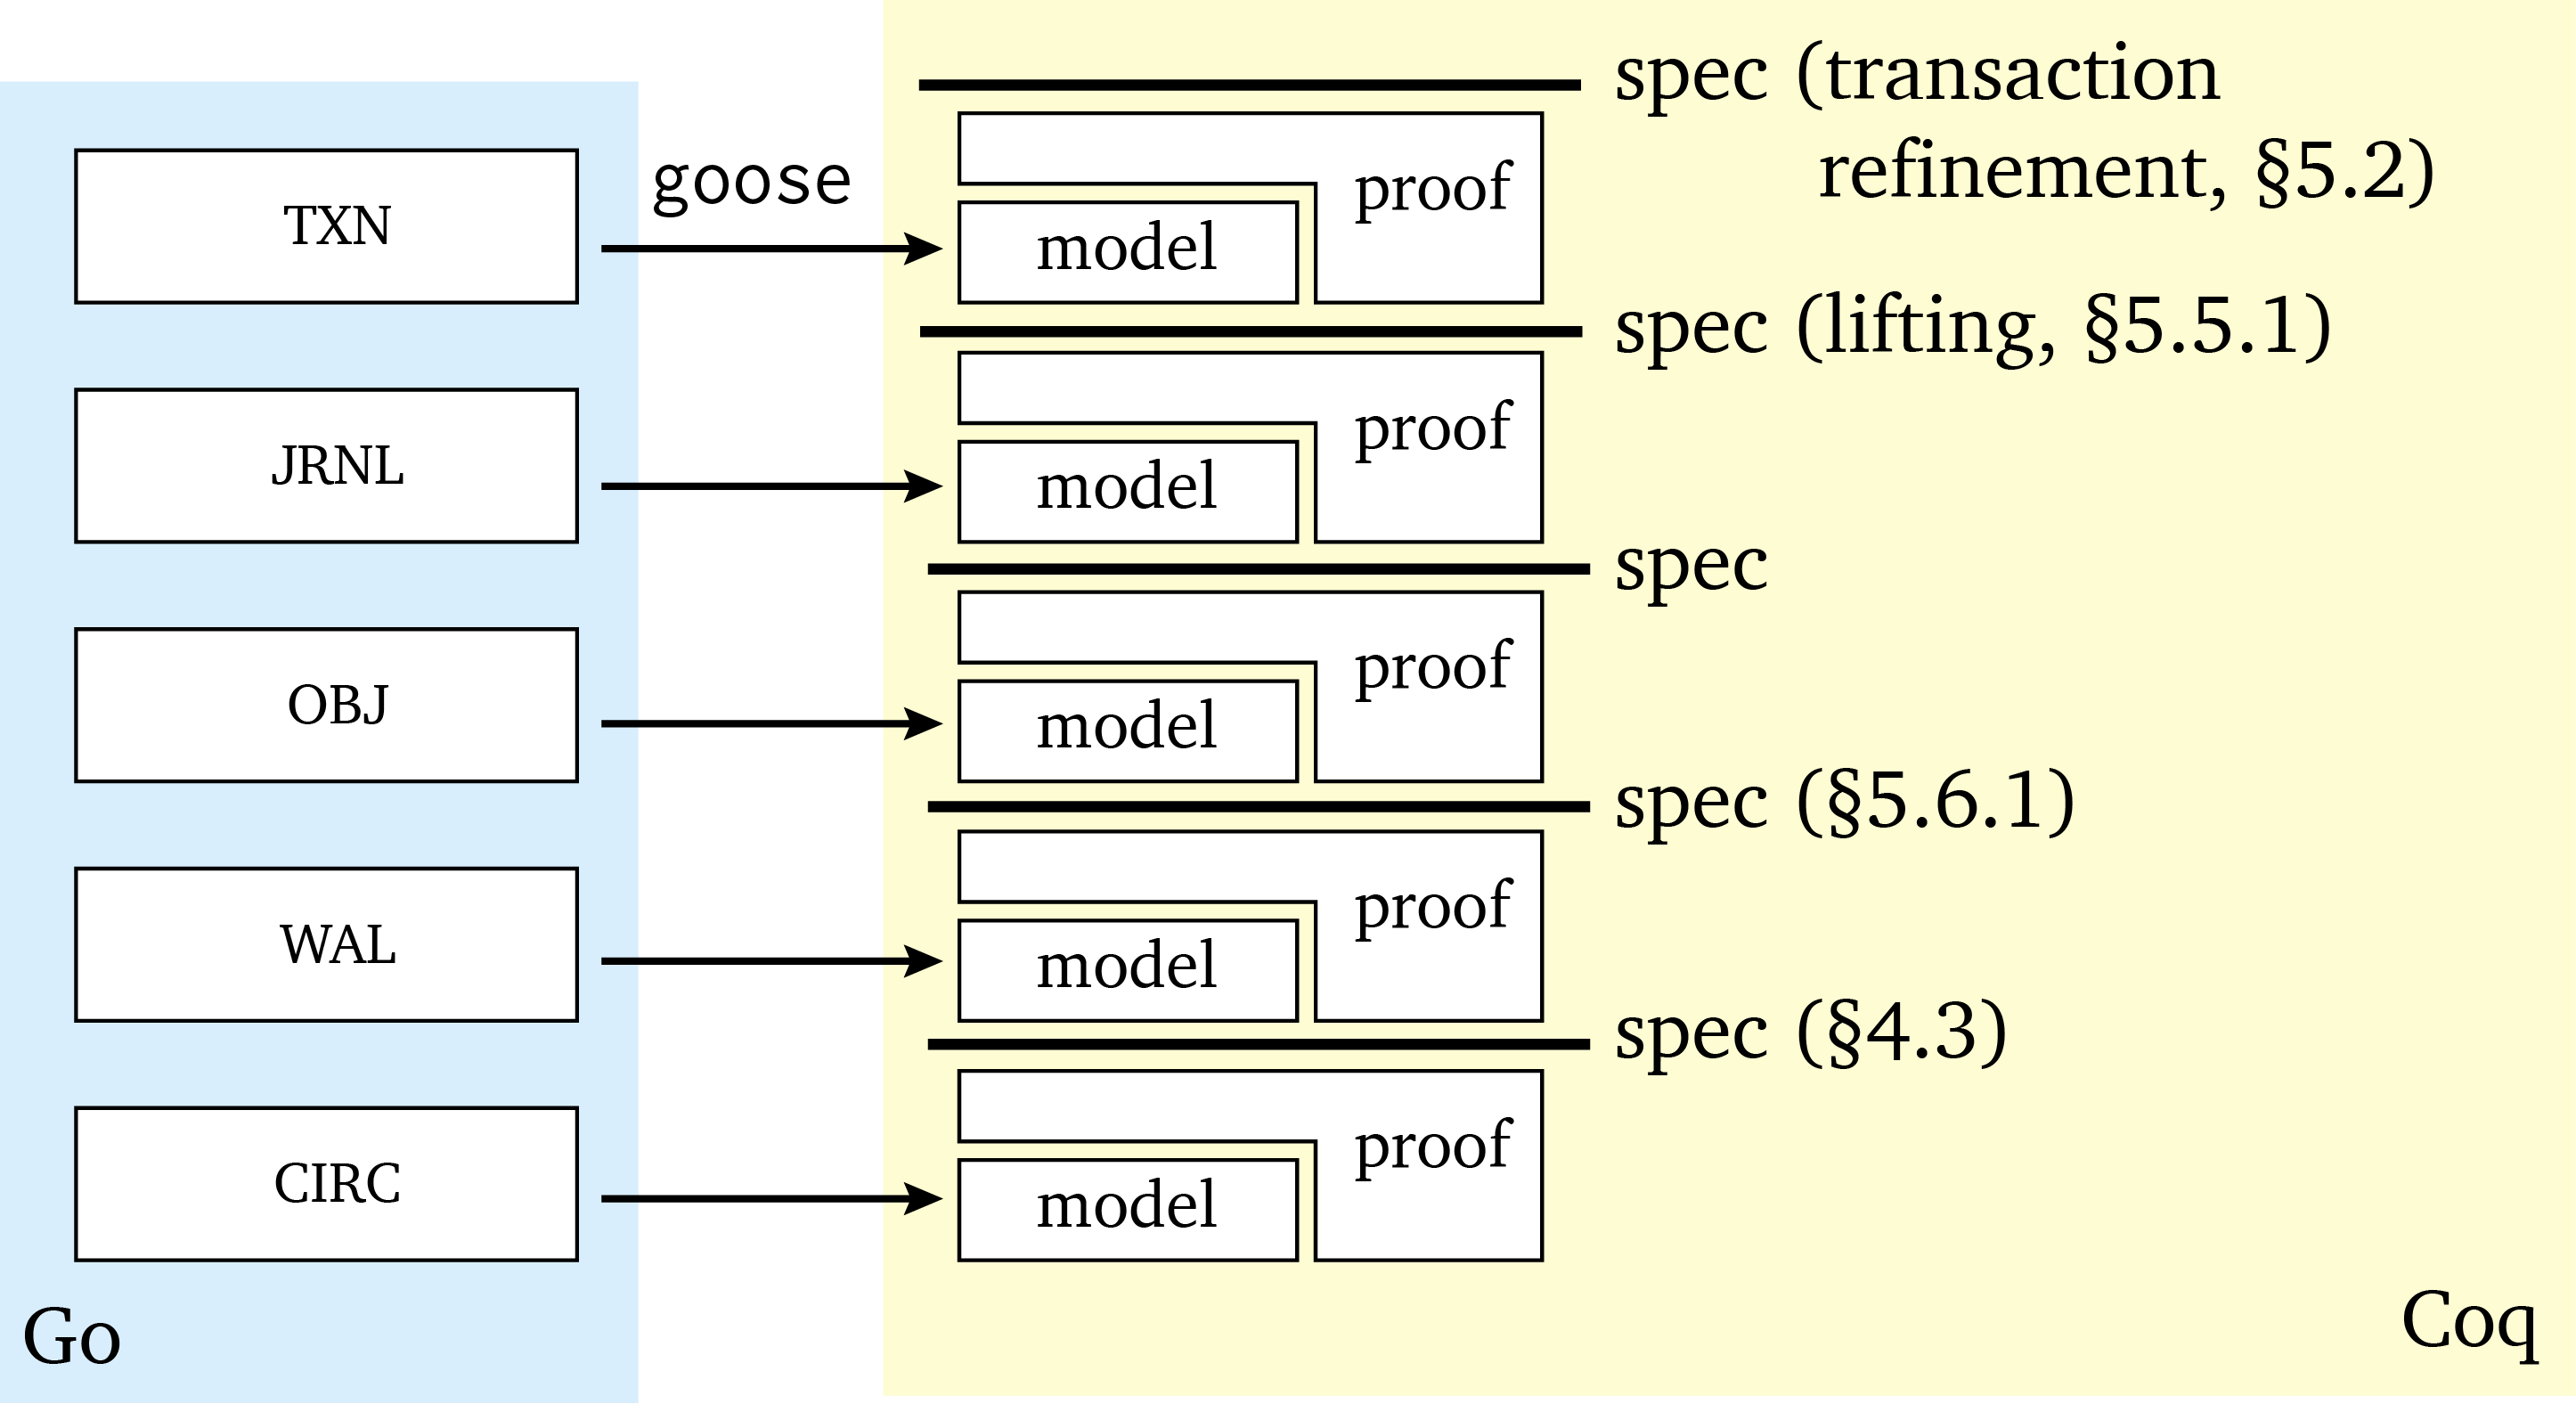
\includegraphics{fig/gotxn.png}
  \caption[Overview of the GoTxn proof layers]%
{Overview of the GoTxn proof, which is divided into proofs for each
    layer. The proofs are all built on top of Perennial.}
  \label{fig:txn:proof-overview}
\end{figure}

\Cref{fig:txn:proof-overview} gives an overview of the libraries (or layers) in
the GoTxn proof. On the left side of the figure is the code, organized into a
stack of libraries, each of which uses the library below. The code is written in
Go and then translated to a model in Coq using Goose (described in
\cref{ch:goose}); each proof is about the model of that library. Each
intermediate layer has a specification which is formally described using
Perennial's logically atomic crash specifications (\scc{txn} has a different
specification). The proofs are all implemented using Perennial for crash safety
and concurrency reasoning, combined with Goose's reasoning principles for Go.

At the bottom level, the \scc{circ} library is implemented using Go primitives
supported by Goose, including an API to access the disk. The disk supports
synchronous reads and writes of 4KB sectors, a standard feature for disk
hardware. On crash, the model of the disk in Perennial assumes writes are atomic
at this 4KB granularity.

At the top level, \scc{txn}'s specification is the transaction refinement
specification described earlier in \cref{sec:txn:spec}. This specification is
about an arbitrary program that uses GoTxn, which is formalized using GooseLang,
the language that we use to model Go code. Note that the statement of transaction
refinement only talks about the GoTxn implementation and a (GooseLang) program
using it; it no longer references the Perennial logic. We are able to prove such
a theorem because Perennial comes with a soundness theorem that relates the
theorems proven using Perennial's crash specifications to the code's execution.
Making the final theorem independent of the logic is important in the next
chapter, \cref{ch:daisy-nfs}, which connects the GoTxn specification to proofs
in Dafny that do not use the Perennial logic.

\section{Verifying atomicity in GoTxn}
\label{sec:txn:proof}

This section outlines the proof of GoTxn's transaction-refinement specification
from \cref{sec:txn:spec}. The implementation consists of multiple layers stacked
together, as described in \cref{sec:txn:impl}. This section focuses on proofs of
the upper two layers: the journaling layer implements \emph{crash atomicity}
while the \scc{txn} layer uses two-phase locking for \emph{concurrency
  atomicity}. The proof is carried out modularly, so the specification for
journaling and the proof of two-phase locking are both described here. The
following section, \cref{sec:txn:lower-layers}, describes aspects of verifying
the lower layers.

Recall that transaction refinement is a statement about an arbitrary program that
uses transactions. It would be infeasible to directly reason about the execution of an
arbitrary use of GoTxn, including handling concurrently issued transactions and
crashes at any time. Instead, the first step is to give a specification to the
individual methods of the GoTxn API, such as \cc{Read}, \cc{Write}, and
\cc{Commit}. Next, the proof considers an arbitrary transaction, but this part
of the proof can now invoke the specifications for each method.

In order to give a specification at the method level, we first
develop the right representation of the intermediate state of a transaction.
This representation needs to capture buffered writes (which will eventually be
durable at commit time) and the old values in the logical disk (which it will
revert to if the system crashes or the transaction aborts). It also needs to
handle concurrent transactions --- the tricky thing here is that the logical
disk can change in the middle of a transaction due to a concurrently committed
transaction, so for example the model of aborts cannot be as simple as reverting
to the disk at the start of the transaction.

A new lifting-based specification for journaling solves these problems. We
introduce a purely logical operation called \emph{lifting} that moves ownership
of a subset of the logical, durable disk into each concurrently executing
transaction. The transaction then operates freely on that part of the disk. This
works because the proof can only lift disjoint parts of the disk, which is
physically guaranteed by using a per-address lock in the \scc{txn} layer.
Eventually the transaction finishes reading and writing, and when it commits any
buffered changes can be merged into the global disk. Aborts are similarly
modeled, returning ownership and merging back the old values of just the local
disk.

% subsection of GoTxn proof section
\subsection{Lifting specification for journaling (\scc{jrnl})}
\label{sec:txn:lifting}

Lifting is defined at an intermediate layer, \scc{jrnl} (for journaling), rather
than for \scc{txn} which is the top-level API of GoTxn. Journaling uses what we
call ``operations'' to distinguish them from ``transactions'' --- an operation
supports reads and writes, and like a transaction can be committed atomically to
disk, but the difference is that the calling library is responsible for guaranteeing
operations manipulate disjoint addresses. In the case of GoTxn, that caller is
the two-phase locking code, whose proof is described in \cref{sec:txn:refinement}.

In the lifting specification, there is a global, logical disk representing the
state of the journaling system, and within each ongoing operation there is a
durable and operation-local view of the disk. The operation-local view is like the disk
view but also incorporates buffered writes. The durable views are disjoint, so
that an address is either in the global disk or ``lifted'' into a particular
operation. Disjointness is what guarantees that the views are really local and
don't change due to concurrent threads.

The lifting-based specification uses a logical concept of ownership to keep all
of these views disjoint and consistent. The state of each view is defined using ghost state
in Iris, and the proof uses separation-logic resources to express ownership over that
ghost state; for a general introduction to the idea of
ownership in separation logic, see \cref{sec:perennial:concurrency}. The
journaling proof issues three types of resources, all per-address:
$a \mapstoDisk o$, $a \mapstoOp o$, and $a \mapstoLftd o$. The first is the most
straightforward: $a \mapstoDisk o$ asserts that the global durable disk has
value $o$ at address $a$ (we use the metavariable $o$ since these addresses have
objects that can be smaller than a block, such as a 128-byte inode value or even
a single bit). In addition, $a \mapstoDisk o$ expresses ownership over the
address $a$. The second resource, $a \mapstoOp o$, asserts ownership of the
operation-local view associated with an in-memory operation $\mathit{op}$; it
mean that either the on-disk value is $o$ or that $\mathit{op}$ contains a
buffered write with the value $o$ to address $a$. The last resource,
$a \mapstoLftd o$ is similar to $a \mapstoDisk o$, but the details are related
to lifting and explained below.


\subsubsection{Initialization}

The first step in using the journaling specification is to initialize the whole
system. Initialization is somewhat complicated by some restrictions GoTxn places
on how sub-block objects are used. The proof requires the caller to fix ahead of
time (when the whole journaling system is initialized) for each block a size for
the objects within. Currently our proofs assume that objects are either a single bit, 128
bytes, or a full block, but supporting an arbitrary power of two should be a
straightforward extension. To initialize the system, the caller supplies a
``schema'' which gives the size of every disk address (that is, every 4KB
aligned address, not the journal's logical sub-block addresses); this enforces
that all the objects within a block are of the same size, which also simplifies
the proof.

The journal's initialization is specified by giving the caller a lemma that
transform ownership over the entire physical disk into the precondition for the
journal's recovery procedure; from this point forward the usual crash and
recovery reasoning in Perennial applies. For each offset $i$ and block size $k$, the initial ownership for that disk
block is just all the objects within that block:
\[
  \operatorname{zeroObjects}(i, k) \defeq \bigast_{0 \leq k \times o < 4096} (i, k \times o) \mapstoDisk 0
\]


The initialization lemma creates resources for all of these initial objects,
starting from an all-zero disk. The lemma takes a schema
$\mathit{kinds}$ that maps disk addresses to block sizes and a disk size $s$;
this schema is arbitrary but fixed at initialization time. We use
$i \mapsto_{\mathrm{disk}} 0$ to denote ownership over a physical disk offset $i$
(not to be confused by the $a \mapstoDisk o$ issued by the journaling proof).
\begin{align*}
  &513 \leq s \land {} \\
  &\operatorname{dom}(\mathit{kinds}) = \{ i \mid 513 \leq i < s \} \land {} \\
  &\bigast_{0 \leq i < s} i \mapsto_{\mathrm{disk}} 0 \wand {} \\
  &\vs \cc{is_txn_crash_condition}(\mathit{kinds}) \sep {} \\
  &\quad \bigast_{(i,k) \in \mathit{kinds}} \operatorname{zeroObjects}(i, k)
\end{align*}

Notice that this initialization is just a logical operation; the schema is not
even required at runtime for the code. It creates \cc{is_txn_crash_condition},
which is the precondition and crash condition for the transaction system's
recovery procedure. The journal objects in this lemma's conclusion are initially
fully owned by recovery, which then shares them with threads. The journaling
system's proof does not fix a particular mechanism for \emph{how} access to these resources is mediated; it
simply requires exclusive access to an address in the form of a
$a \mapstoDisk o$ resource. In practice, GoTxn mediates access to
$a \mapstoDisk o$ by protecting it with a per-address lock. In our paper on the
journaling system itself we wrote a proof of a simple file system where the
locks were instead per inode, so that one lock protected more than one journal
resource; see the GoJournal paper for details on that use
case~\cite{chajed:gojournal}.

\subsubsection{Preparing operations}

The specification for \cc{Begin()} is straightforward, since the operation has
not yet interacted with the disk:
\hypertarget{tgt:begin-spec}{}
%
\begin{align*}
  \hoareV{\TRUE}%
  {\cc{Begin}()}%
  {\Ret{op} \cc{is_op}(\mathit{op})}
   %\tagH{BeginSpec}
\end{align*}
The specification has a trivial precondition of $\TRUE$ and its postcondition
returns an assertion \cc{is_op}, which says that $\mathit{op}$ is a valid
\cc{*Op} object that represents a journaling operation.  (This is different from
the \cc{*Txn} object that represents for a transaction, which has additional
state to track locking.) The operation starts out with an empty operation-local
view and ownership over no addresses; the ghost state for this operation's view
is initialized by the proof of this theorem and represented as part of
$\cc{is_op}(\mathit{op})$.

In order to interact with an address within an operation, the specification
requires the caller to start with $a \mapstoDisk o$ and then \emph{lift} it to
obtain an operation-local resource, where lifting is the following purely
logical operation:
\[
  a \mapstoDisk o \vs a \mapstoOp o \sep a \mapstoLftd o
\]

Notice that the result of lifting is both an operation-local assertion and
$a \mapstoLftd o$; this latter assertion is much like $a \mapstoDisk o$ in that
it asserts the on-disk value of address $a$, but it cannot be lifted again. This
is required for soundness; only one of $a \mapstoDisk o$ and $a \mapstoOp o$ is
allowed for ownership to actually be exclusive. Not shown is that lifting does
also require $\cc{is_op}(\mathit{op})$ which reflects that the ghost state has
been set up.

The specification for \cc{OverWrite} describes the effect of writing to the
local memory of a buffered journal operation:
%
\begin{align*}
  \hoareV{\cc{is_op}(\mathit{op}) \sep a \mapstoOp o \sep \cc{buf_obj}(buf, o')}%
        {\mathit{op}.\cc{OverWrite}(a, buf)}%
        {\cc{is_op}(\mathit{op}) \sep a \mapstoOp o'}
  %\tagH{OverWriteSpec}
\end{align*}

The precondition includes $\cc{buf_obj}(buf, o')$ to say that the in-memory
buffer $buf$ encodes the object to be written $o'$.
The \cc{is_op} predicate is both
required and returned by the specification, which reflects the fact that
\cc{OverWrite} operates on the in-memory and ghost state covered by
this predicate.

The specification for \cc{ReadBuf} is similar. \cc{ReadBuf}
returns a buffer that points into the \cc{op} struct, so it has a more
sophisticated spec:
%
\begin{align*}
  \hoareV{\cc{is_op}(\mathit{op}) \sep a \mapsto_{\mathit{op}} o}%
        {op.\cc{ReadBuf}(a)}%
        {\Ret{buf}
  \begin{aligned}
  &\cc{buf_obj}(\mathit{buf}, o) \sep \phantom{} \\
  &\quad( \cc{buf_obj}(\mathit{buf}, o) \wand \\
  &\quad\quad \cc{is_op}(\mathit{op}) \sep a \mapsto_{\mathit{op}} o )
    \end{aligned}}
    %\tagH{ReadBufSpec}
\end{align*}

This states that, when \cc{ReadBuf} finishes, it returns a buffer $\mathit{buf}$
and two resources: $\cc{buf_obj}(\mathit{buf}, o)$ says the buffer has the old
object $o$, while the second is a separating implication or \emph{wand} $\wand$.
The wand says that if
the caller returns ownership of $\cc{buf_obj}(\mathit{buf}, o)$, it can get back
the $\cc{is_op}(\mathit{op})$ predicate. This allows the caller to use the
buffer to read the data before continuing to read and write within the
operation. The complete specification in GoJournal also supports modifying the
object using the buffer returned by \cc{ReadBuf}~\cite{chajed:gojournal}, but
GoTxn does not expose that feature.

\subsubsection{Commit}

The final method in the journaling API is \cc{Commit()}, which atomically
persists all the writes buffered in the operation. The specification is based on
two maps $m$ and $m'$ whose domains are the set of all addresses lifted into the
operation. The first map $m$ gives the on-disk, pre-operation values while $m'$
has the new values buffered in the operation.
\begin{align*}
  \hoareCV{ \begin{aligned}
              &\dom(m) = \dom(m') \sep {} \\
  &\left( \bigast_{(a,o) \in m} a \mapstoLftd o \right) \sep %
  \left( \bigast_{(a,o') \in m'} a \mapstoOp o' \right)
            \end{aligned}} %
  {\mathit{op}.\cc{Commit}()}%
  {\Ret{\mathit{ok}} \mathrm{if~} \mathit{ok} %
  \mathrm{~then~} \bigast_{(a,o') \in m'} a \mapstoDisk o' \mathrm{~else~} %
    \bigast_{(a,o) \in m} a \mapstoDisk o}%
  {\left( \bigast_{(a,o) \in m} a \mapstoDisk o \right) \lor
    \left( \bigast_{(a,o') \in m'} a \mapstoDisk o' \right) }
\end{align*}

The precondition in this specification requires ownership over a subset of the
logical disk given by $\dom(m) = \dom(m')$, both its durable values and the
operation-local view. If the system does not crash and returns
$\mathit{ok} = \goosetrue$, \cc{Commit} returns ownership over the new values
on disk. It returns full disk points-to assertions $a \mapstoDisk o'$ because
these addresses are ``lowered'' so that subsequent operation can lift them
again. If the commit aborts (which only happens if the transaction does not fit
in memory), then the specification still returns full disk ownership albeit with
the old values. The crash condition of the \cc{Commit} specification captures
that even if the system crashes, it still returns ownership over the disk
resources, with either the old or new values. Whether this disjunction goes to
the left- or right-hand side depends on exactly when the system crashes; see
\cref{sec:perennial:recovery-spec} for a discussion of how the proof handles
this.

It's a little easier to see the overall structure of \cc{Commit}'s specification
if we specialize it to a single address (although the specification is powerful
because it captures atomicity across multiple addresses):
\begin{align*}
  \hoareCV{a \mapstoLftd o \sep a \mapstoOp o'} %
  {\mathit{op}.\cc{Commit}()}%
  {\Ret{\mathit{ok}} \mathrm{if~} \mathit{ok} %
  \mathrm{~then~} a \mapstoDisk o' \mathrm{~else~} a \mapstoDisk o}%
  {a \mapstoDisk o \lor a \mapstoDisk o'}
\end{align*}

% subsection of GoTxn proof section
\subsection{Refinement to atomic language}
\label{sec:txn:refinement}

\newcommand{\txnmapsto}{\mapsto_{\cc{txn}}}
\newcommand{\thdmapsto}{\Rightarrow}

Recall that \cref{thm:gotxn-program-refinement} is the overall correctness
theorem for GoTxn. It says that the GoTxn implementation is a \emph{program
refinement} between the Txn layer (with programs that use transactions) and the
Disk layer (with an implementation that interacts with a disk).
That is, given a program
$p : \gooselayer{Txn}$, if the transaction operations of $p$ are linked with
GoTxn (implemented in $\gooselayer{Disk}$), the implementation program's
observable behaviors (from running on a disk) are a subset of the
specification's behaviors (with high-level transaction-system operations, and in
particular atomicity for transactions). The proof of this theorem leverages the
journaling specification from \cref{sec:txn:lifting}, extending it to also
reason about the concurrency control implemented with two-phase locking.

In general, the Perennial framework supports proving refinements between a
specification layer $\gooselayer{S}$ and an implementation layer $\gooselayer{I}$ by constructing
a simulation between the specification and its implementation. The simulation is
expressed in terms of refinement conditions that are written using the usual
Perennial Hoare triples specifications (with pre- and postconditions),
so that they can be proven using the full spectrum of techniques in Perennial.

Following an
approach developed by \citet{turon:caresl}, in a refinement proof in Perennial the execution of the specification
program is represented by \emph{ghost state}. The logic then has assertions for
describing this ghost state.  For example, for the Txn layer, the assertion $\cc{a}
\txnmapsto b$ says that address $a$ contains the value $b$ in the ghost
transaction system's state. In addition, there are \emph{thread points-to}
assertions, written $j \thdmapsto \cc{e}$, which says that thread $j$ in the
specification program is executing program $\cc{e}$. Perennial has rules
for updating the ghost state by ``executing'' these ghost threads, such as the
following view shift:
\[
  (\cc{a} \txnmapsto b) \sep (j \thdmapsto \cc{Write(a, b')}) \vs
  \cc{a} \txnmapsto b'
\]
which updates the value stored at $\cc{a}$ as a result of a write.

To establish the refinement, the proof engineer first defines a
\emph{representation invariant} $I$, an assertion in the logic that describes a
relation between the specification state and the implementation state.
Perennial's proof rules ensure that this designated invariant must hold before
and after each step of a program throughout the proof. Next, the proof engineer
proves a Hoare triple for each operation $o$ of $\gooselayer{S}$ and its
corresponding implementation $p_o$ in $\gooselayer{I}$:
\[
\hoare{(j \thdmapsto o) * \knowInv{}{I}}{p_o}{\Ret{v} (j \thdmapsto v)}
 \]
Such a \emph{refinement triple} says that if a specification thread is executing
$o$ and an implementation thread is running $p_o$, then the representation
invariant $I$ is maintained and the value $v$ returned by running $p_o$ is a valid
return value of operation $o$. In the proof of this triple, the ghost execution
rule above is used at the linearization point of $p_o$, to mark
when the operation logically takes effect by executing $o$ in the ghost code.

These refinement triples imply a refinement between programs in $\gooselayer{S}$
and $\gooselayer{I}$. This is formally stated and proven in Coq, using the Perennial
framework's soundness theorem.

In the particular case of the transaction system, the key refinement triple to
prove is for a block of code $f$ enclosed in transaction \cc{Begin} and
\cc{Commit} operations; for example the triple might look the following (for a
particular transaction $f$ that copies from address 0 to 1):
\[
  \hoareV{ \left( j \thdmapsto %
      \atomically{v \gets \mathit{Read}(0);\, \mathit{Write}(1, v)} %
    \right) %
    \sep \knowInv{}{I}}%
  {\begin{aligned}
&\cc{tx := Begin();} \\
&\cc{v := tx.Read(0); tx.Write(1, v);} \\
&\cc{tx.Commit()}
\end{aligned}}%
    {j \thdmapsto ()}
\]
The difficulty in proving this triple is that the linearization point is at the
very end when the code calls \cc{Commit}, at which point the actual earlier
execution of $f$ becomes visible to other threads. The proof must show that
ghost-executing the specification's \cc{atomically} block at this point is valid by
tracking the behavior of $f$.

\tej{approximately here explain how the lock invariants are set up to protect
  the GoJournal disk resources and their crash invariants}

To show this, our proof maintains a stronger invariant during a transaction's
execution. As the transaction executes, we track the initial, on-disk value of any
objects accessed in a map $J$. The domain of this map
$\Sigma = \operatorname{dom}(J)$ is the \emph{footprint} of the transaction,
which two-phase locking keeps locked during the transaction. The intuition
behind the invariant is that if the transaction only depends on $J$, the
transaction's execution can be delayed to take place atomically at the call to
\cc{Commit} and its behavior will be the same since the subset of the journal
$J$ is the same.

The proof needs to reason about the two-phase locking concurrency control in
order to use the journaling layer's lifting specification as part of this proof.
Perennial has a crash-aware specification for locks, described in
\cref{sec:perennial:wpc}, that allows us to reason about the per-address locks
while also reasoning about crashes in the middle of a transaction. To use this
specification, the proof defines a per-address lock invariant and crash
invariant --- the lock invariant is a property that holds when the lock is
acquired (and must be shown when it is released), while the crash invariant is a
guarantee that also holds on crash. In the case of the two-phase locking code,
both the lock and crash invariants for the lock associated with address $a$
contain ownership of $\exists o, a \mapstoDisk o$, which gives the transaction
the ability to lift address $a$ and read and write it with the journaling
system's interface. The invariant has additional constraints to assert that the
value $o$ is the same as the one in the transactional disk.

More formally, the proof constructs a second simulation relation during the
execution of a transaction $\cc{f}$.  Let $J$ be a map giving the values of each
object in the transaction's footprint $\Sigma$ at the first time they are
accessed by $\cc{f}$, and let $J'$ be a mapping giving the transaction's current
buffered in-memory view of the same addresses.  Then, the invariant requires
that after $n$ steps of execution:
%
\begin{enumerate}

\item The transaction holds the lock for every address $a \in \Sigma$. The
transaction has ownership over $\bigast_{(a,o) \in J} a \mapstoLftd o$ due to
holding these locks and $\bigast_{(a,o') \in J'} a \mapstoOp o'$ from the
buffered writes.

\item Executing $n$ steps of $\cc{f}$ in \emph{any} starting state that has the same
  values as $J$ for the addresses in $\Sigma$ can lead to a state with values given
  by $J'$.

\end{enumerate}
%
At the start of a commit, the locking described by the first part of the
invariant ensures that the durable value of each address still match the values
in $J$. The second part of the invariant means that even though other
parts of the state outside of $\Sigma$ may have changed, those changes do not
affect execution of $\cc{f}$. Thus, the ghost execution of $\cc{f}$ at this point will
have the same behavior as the implementation. The transaction's invariant
maintains ownership of the resources to use the journal's \cc{Commit}
specification. The postcondition and crash condition of that specification
return new disk points-to assertions consistent with either $J$ or $J'$ as
appropriate. If the commit is successful, then the second part of the
transaction system's invariant allows issuing a ghost-execution update to change
the transactional disk from $J$ to $J'$ (for the subset $\Sigma$), and it
guarantees that this correctly simulates \cc{f}.

Showing that the second part of the invariant holds requires that code within a
transaction must not access global state outside of the
transaction system, as mentioned in \cref{sec:proof:linking}. Accesses to such global state
would violate the invariant because their behavior would then depend upon
things outside of the footprint $\Sigma$. Because those global values could change
by the time the transaction commits, the above argument would no longer work if they were allowed.

The allocator creates another subtlety related to the second part of this
invariant. Allocations do not hold the allocator lock throughout the remainder
of a transaction. This seems to violate the two-phase locking pattern, since
allocations could be implicitly observed by other concurrent transactions from
the fact that an allocated address is no longer free. Correspondingly, in the
proof, the footprint $J$ of a transaction does not describe the allocator state.
Thus, at the ghost-execution linearization point, the addresses returned by the
allocator may no longer be free. However, because the specification for the
allocator does not guarantee that returned addresses are actually free, the
second part of the invariant above still holds.

% Suppose the transaction being simulated is $\operatorname{Atomically}{f}$, and the implementation
% has executed $n$ steps of $f$, accessing addresses in the set $\sigma$.

% Let $J_1 : \cc{addr} \rightarrow Obj$ be a map giving the durable state of the journal at the start of the transaction, and let $J_2$ be the current buffered in-memory view of the state from the perspective of the transaction.
% Then, the invariant requires that:
% \begin{enumerate}
% \item the transaction holds the lock for every address $a \in \sigma$
% \item for each $a$, $J_1(a)$ matches the ghost state value for the address $a$
% \item if $J_1'$ is a mapping such that $\forall a \in \sigma$, $J_1(a) = J_1'(a)$, then executing $f$ for $n$ steps with an initial journal $J_1'$
% \end{enumearte}
% \joe{this would probably be vastly improved by using math notation that matches whatever will have been used in the previous two sections}


\section{Verifying GoTxn's implementation layers}
\label{sec:txn:lower-layers}

This section walks through the proof of lower layers of GoTxn's implementation.
Rather than give complete specifications and proof sections, it focuses on some
of the most interesting aspects.

\subsection[Write-ahead logging (WAL)]{Write-ahead logging (\scc{wal})}
\label{sec:txn:wal}

The write-ahead log layer is responsible for updating multiple disk
blocks (a multiwrite) atomically.
Each multiwrite is a list
of updates, where an update consists of a disk block number and the new data to write in that block.
%The write-ahead log makes transactions atomic by first writing the
% updates to an on-disk log, and then installing them to their respective
% disk blocks.
A background logger thread moves multiwrites from an in-memory buffer to an
on-disk log. To make this atomic, the logger first writes
the contents of a multiwrite in a log entry, and then updates a designated header block to indicate
the entry is complete. If a crash
happens before the header is updated, none of the multiwrite's updates
are applied; if a crash happens after the header update, the multiwrite
will be applied during recovery.
Meanwhile, an installer thread applies entries in the log to the disk, clearing
space for new multiwrites.
If a crash happens before the updates in an entry are fully installed,
recovery installs the updates again from the on-disk log.

The write-ahead log implements two optimizations related to combining
multiwrites. Two or more multiwrites can be \emph{group committed} by logging
them together, which still guarantees their atomicity. If multiwrites being
committed together update the same block, the first update can be
\emph{absorbed} and replaced with the second. These optimizations trigger both
for multiwrites that are committed without waiting for durability and also for
concurrent, synchronous multiwrites.

% When a transaction is written in the log,
% updates to the on-disk log is made atomic by first writing the updates
% to the log, and then updating a designated header block.
%
% If a crash
% happens before the header is updated, none of the transaction's updates
% are applied; if a crash happens after the header update, the transaction
% will be applied during recovery.

% Write-ahead logging is a standard approach for atomic disk writes, but it
% is complicated by performance and crash safety requirements.  For example,
% writing transactions to disk requires waiting for a disk write, which
% can be slow.  To improve performance, many storage applications do not
% flush transactions to disk immediately (e.g., unstable \scc{write} RPCs
% in NFSv3), but do require that the on-disk state be consistent (i.e.,
% no partially applied or out-of-order transactions) after a crash.
% Furthermore, because disk writes are slow, many operations need to
% happen in parallel, without holding locks while waiting for disk reads
% and writes: committing new transactions in memory; logging transactions
% from memory to disk; waiting for transactions to be made durable; and
% installing transactions.  Concurrency ensures that in-memory operations
% need not wait for any in-flight disk reads or writes, and that many
% disk reads and writes can happen at the same time.  Finally, to reduce
% the number of disk writes, multiple in-memory transactions are logged
% to disk together (``group commit''), and if they update the same disk
% block multiple times, only the most recent update of that disk block is
% written to the log (``absorption'').

% Formally verifying a high-performance write-ahead log is challenging
% because of the lock-free concurrency, and because the log must maintain
% crash-safety at all times.


\paragraph{Internal abstract state: logical log.}
To prove the write-ahead log layer correct, the proof represents the
state of the write-ahead log as a logical list of multiwrites, as
shown in \cref{fig:log}.  Multiwrites before \cc{memStart} have
already been installed, and their log entries do not physically exist in memory or on disk.
Multiwrites from \cc{memStart} to \cc{diskEnd} are already logged on
disk.  Multiwrites from \cc{diskEnd} to \cc{nextDiskEnd} are currently being logged
from memory to disk.  Finally, multiwrites between \cc{nextDiskEnd}
and \cc{memEnd} are purely in-memory, and are eligible for absorption.

\begin{figure}[ht]
  \centering
    \begin{tikzpicture}[>=latex]

  \tikzstyle{log}=[thick,rectangle, draw, minimum width=3cm,minimum
    height=1.5cm, align=center,fill=blue!10];

  \node[log] (installed) {Installed \\ writes};
  \node[log,right=0cm of installed] (logged) {Logged \\ writes};
  \node[log,right=0cm of logged] (logging) {Writes being \\ logged};
  \node[log,right=0cm of logging] (unstable) {Unstable \\ writes};

  \node[] at (-1.3cm, -1cm) {$\uparrow$ 0};
  \node[] (memstart) at (2.2cm, -1cm) {$\uparrow$ \cc{memStart}};
  \node[] (diskend) at (5.2cm, -1cm) {$\uparrow$ \cc{diskEnd}};
  \node[] (nextdiskend) at (8.55cm, -1cm) {$\uparrow$ \cc{nextDiskEnd}};
  \node[] (memend) at (11.1cm, -1cm) {$\uparrow$ \cc{memEnd}};

  \node[font=\footnotesize, below=0cm of memstart, align=center, xshift=-0.6cm] {Advanced by \\ installer};
  \node[font=\footnotesize, below=0cm of diskend, align=center, xshift=-0.5cm] {Advanced by \\ logger};
  \node[font=\footnotesize, below=0cm of nextdiskend, align=center, xshift=-0.85cm] {Advanced by \\ \cc{Flush}};
  \node[font=\footnotesize, below=0cm of memend, align=center, xshift=-0.5cm] {Advanced by \\ \cc{Commit}};

\end{tikzpicture}

    \vspace{0.5 \baselineskip}
    \caption{The logical write-ahead log.  Vertical arrows indicate
        designated positions in the logical log.  Labels below the arrows
        indicate what thread or function is responsible for advancing
        that logical position to the right.}
    \label{fig:log}
\end{figure}

This representation allows the WAL's proof to precisely specify how concurrent
operations modify this abstract state, and how the state changes on crash.
For example, although the installer thread performs many disk writes to
install multiwrites, its only effect on the abstract state is that it
advances \cc{memStart}.  Similarly, the logger thread's only change to
the abstract state is to advance \cc{diskEnd}.  Calling \cc{Flush()}
advances \cc{nextDiskEnd}, freezing the data to be logged, then waits
for the logger to advance \cc{diskEnd} up to that point.  Committing a
new multiwrite simply appends it at \cc{memEnd}.  Finally, on crash,
an arbitrary suffix of the log from \cc{diskEnd} onwards is discarded.


\paragraph{External abstract state: durable lower bound.}
Although the details of the logical log are important for proving the
\scc{wal} layer, the caller (i.e., the \scc{obj} layer) does not need
to know about installation, group commit, etc. To abstract away these
details, the \scc{wal} provides a simplified state as its interface,
as shown in \cref{fig:wal-spec}.  The simplified state consists of
the same list of multiwrites, together with \cc{durable_lb}, which is
a lower bound on what set of multiwrites will be preserved on crash.
Using a lower bound instead of precisely exporting \cc{diskEnd} means
that this abstract view does not need to change if the logger thread
adds more multiwrites to disk in the background, and thus hides
this concurrency.

\begin{figure}[ht]
  \begin{minted}{coq}
Record update := { addr: u64; data: Block; }.
Record State :=
  { multiwrites: list (list update);
    (* at least durable_lb elements are durable *)
    durable_lb: nat; }.

Definition mem_append (ws: list update) :
    transition State unit :=
  modify (set multiwrites (fun l => l ++ [ws]));
  ret tt.

(* non-deterministically pick how many
   multiwrites survive the crash. *)
Definition crash : transition State unit :=
  durable <- suchThat (fun s i => durable_lb s ≤ i);
  modify (set multiwrites (fun l => l[:durable]));
  modify (set durable_lb (fun _ => durable));
  ret tt.
  \end{minted}
\caption{Parts of the specification for the \scc{wal} interface.}
\label{fig:wal-spec}
\end{figure}


\paragraph{Lock-free logging and installation.}
For performance, GoTxn has dedicated threads that perform logging and
installation.  However, these threads do not hold any locks while reading
or writing to disk.  To allow these threads to run concurrently, the write-ahead
log layer
uses two separate header blocks, as shown in \cref{fig:physlog}.
One header block (owned by the installer thread) stores the start of
the on-disk log, and another header block (owned by the logger thread)
stores the end of the on-disk log.  This lets the installer and logger
concurrently advance their pointers (\cc{memStart} and \cc{diskEnd}
respectively) without locks.

\begin{figure}
    \centering
    \begin{tikzpicture}[>=latex]

  \tikzstyle{circlog}=[thick,rectangle, draw,minimum height=1.5cm, align=center,fill=magenta!10];
  \tikzstyle{log}=[thick,rectangle, draw,minimum height=1.5cm, align=center,fill=green!10];

  \node[circlog,minimum width=1cm] (logger) {Logger \\ end \\ pointer};
  \node[circlog,minimum width=1cm, right=0cm of logger] (installer) {Installer \\ start \\ pointer};

  \node[circlog,minimum width=2cm, right=0cm of installer] (log) {Logged \\ multiwrites};

  \node[log,minimum width=3cm, right=0cm of log] (log) {Installed \\ blocks};

  \node[] at (-0.45cm,-1cm) {$\uparrow$ 0};
  \node[] at (4.2cm,-1cm) {$\uparrow$ 513};

  \draw [decorate,decoration={brace,mirror,amplitude=10pt},xshift=-4pt,yshift=0pt]
    (-0.45cm,-1.2cm) -- (4cm,-1.2cm) node [black,midway,yshift=-0.6cm]
    {\scc{circular}};

\end{tikzpicture}

    \caption{The physical write-ahead log.}
    \label{fig:physlog}
\end{figure}

Although the logger and installer threads can perform lock-free disk
writes, they must still coordinate with one another.  For example,
the installer cannot run ahead of the logger thread, and the logger
thread must coordinate with threads that are appending new multiwrites
in memory. GoTxn's proof uses the notion of \emph{monotonic counters} to reason
about the safety of the logger and installer's lock-free operations.

The logger thread needs to check that \cc{memStart} is far enough along that the
log will have space for the new multiwrite. The proof gets a \emph{lower bound}
on the \cc{memStart} variable while holding a lock, which remains true even
after releasing the lock. Even though \cc{memStart} might grow after the initial
check, the log will only have more space and thus the multiwrite will still fit.

The installer has a similar lock-free region that also reasons using a lower
bound. The installer retrieves the updates from the current \cc{memStart} to
\cc{diskEnd} in order to start installing them to disk. When the installer
eventually trims the log, it needs to be sure not to advance beyond the current
logger position, which the proof demonstrates using a lower bound on
\cc{diskEnd} from when the logger initially started.

The proof of this aspect of the write-ahead log is one of the trickiest parts of
GoTxn, because of the lock-free concurrency in the write-ahead log. For more
details on the proof strategy, see Mark Theng's thesis~\cite{mtheng-meng}. Mark
helped complete the proof and described the complete proof and its invariants in
more detail in his thesis.

\paragraph{Specifying lock-free reads.}
Concurrency in the write-ahead log complicates not just its proof but its
specification due a challenge with reading installed data. The difficulty is that
reading requires checking the log's in-memory cache and then falling back to the disk,
but the disk read happens without a lock. If a multiwrite commits after the read
misses in the cache, then the disk read will not observe the latest value. The
write-ahead log specification specifies that reading the installed value might return an
old view of the disk, and the \scc{obj} layer above handles this weaker specification with
an invariant that guarantees the object being read has not been modified since
that old view.

More concretely, \cref{fig:walread} shows the implementation of \cc{Read} in the
\scc{wal} layer.  This implementation is split into two parts. The first part checks
the in-memory state by consulting \cc{l.memLog} under a lock (line 9), checking for any
updates to the address being read between \cc{memStart} and \cc{memEnd}. If
no in-memory updates match the address being read, the second part of \cc{Read} falls back
to reading from the installed area on disk (line 15).  No single lock is held across the whole
operation, so other threads
can run between the call to \cc{ReadMem()} and \cc{ReadInstalled()} across lines
2--4.
In particular, a thread could run \cc{Commit()}
to the same block that another thread is reading, if the two threads
are accessing different parts of the same block, as shown in \cref{fig:txn-concur}.

\begin{figure}[ht]
\begin{minted}[linenos]{go}
func (l *Wal) Read(a uint64) Block {
  b, ok := l.ReadMem(a)
  if ok { return b }
  return l.ReadInstalled(a)
}

func (l *Wal) ReadMem(a) (Block, bool) {
  l.Lock()
  b, ok := l.memLog.get(a)
  l.Unlock()
  return b, ok
}

func (l *Wal) ReadInstalled(a uint64) Block {
  return disk.Read(a)
}
\end{minted}
\caption{The implementation of \cc{Read} in the \scc{wal} layer.}
\label{fig:walread}
\end{figure}

There is a challenge in specifying the behavior of \cc{Read} because its commit
point is not obvious. Consider a case
where address $a$ is not in the in-memory log, so that the \cc{Read} operation
falls back to \cc{ReadInstalled(a)} --- the situation is depicted graphically in
\cref{fig:wal:future-read}. If there is a concurrent write to address
$a$, then there are two possibilities for the linearization point of the
\cc{Read} call: it can either appear to occur before the concurrent write, if
\cc{ReadInstalled(a)} returns the old value, or its linearization point might be
after the write if the concurrent write is installed before
\cc{ReadInstalled(a)} runs. Unfortunately the decision to linearize before
\cc{ReadInstalled(a)} or at the point it runs \emph{depends on the future
  behavior} of the system (the linearization point is before if there is no
concurrent write that gets installed, but if there is such an installed write it
needs to be after that write).

\begin{figure}[ht]
  \centering
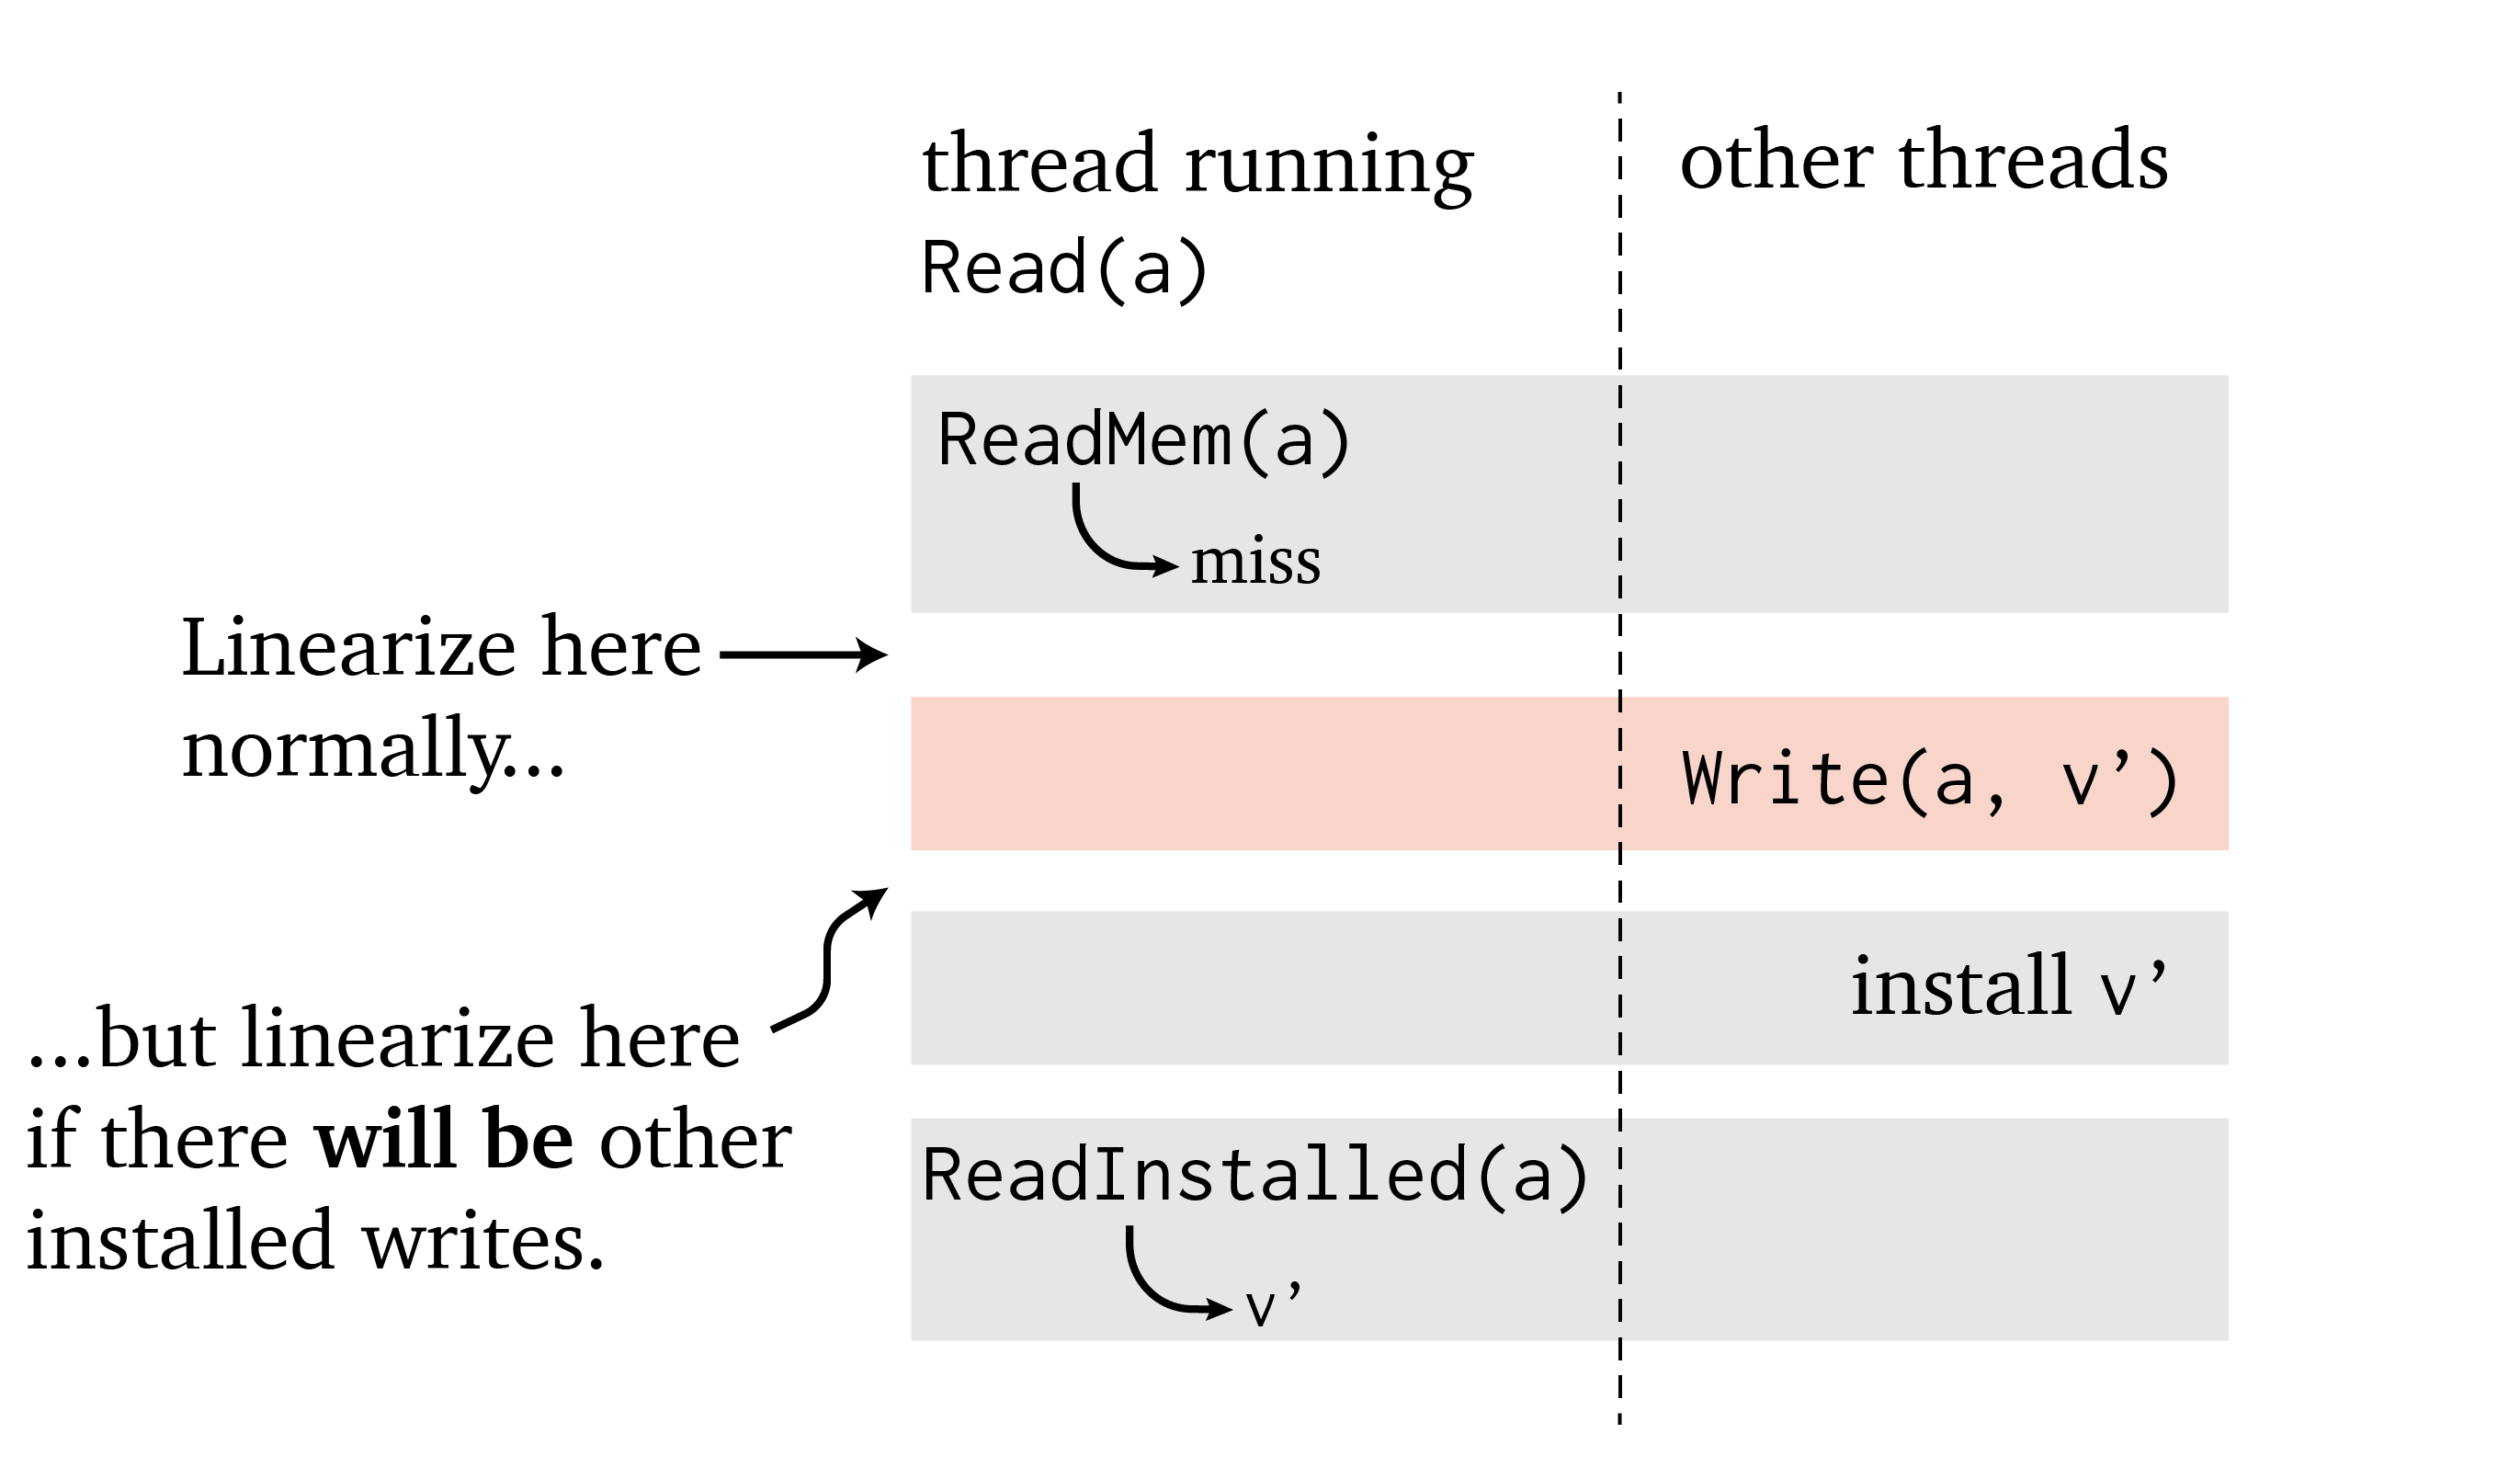
\includegraphics{fig/future-read.png}
\caption[Future-dependent linearization point for WAL's Read operation]{The
linearization point for \cc{Read(a)} depends on future operations. In
this example, there is a concurrent write to the address being read
(highlighted in red). Because this write is installed before the
\cc{ReadInstalled} operation, the correct linearization point is after the read,
but if the installation had not happened yet the \cc{Read} would return the old
value and the linearization point is earlier.}
\label{fig:wal:future-read}
\end{figure}

Instead of proving that \cc{Read} is atomic, we instead give atomic specifications to
\cc{ReadMem()} and \cc{ReadInstalled()} individually. The write-ahead log's
abstract state includes a lower bound on its installed point in order to
describe \cc{ReadInstalled()} in isolation. The specification for \cc{ReadMem}
if the address is not in the log says that it
advances the installed lower bound enough to guarantee that there are no writes
to that address after the new installed point. The specification for
\cc{ReadInstalled()} can return any value the address has after the
installed lower-bound. To reason about the combination of these operations, the
\scc{obj} layer maintains a strong invariant about all the possible blocks that
\cc{Read} could return from the installed point onward, and this is enough to
reason about a block returned from either the cache or the installed data.

Formally, we believe that it is possible to prove that the \scc{wal} \cc{Read()}
operation is linearizable, but because of the future-dependence this
will require using \emph{prophecy variables}.  Perennial
does not support them, which forced us to adopt the non-atomic
specification described above.  Recent results on prophecy variables
in Iris~\cite{jung:prophecy} could be used to avoid specifying
\cc{ReadInstalled()} separately.

\subsection{Logically atomic crash specifications}
\label{sec:txn:logatom}

Throughout the GoTxn stack we specify internal layers using a transition-system
specification, such as the examples illustrated in \cref{fig:wal-spec} for
the \scc{wal} layer. Perennial formalizes what it means for the code in a layer to
implement a transition system in terms of Perennial's crash triples in a style we call
\emph{logically atomic crash specifications}. \Cref{ch:crash-logatom} gives a
more complete description of this encoding. This section gives the high-level
intuition for how these specifications are used in the context of the GoTxn
layers.

As a motivating example, consider the moment when the logger thread commits a
new batch of multiwrites to the physical log in order to advance the durable
point \cc{diskEnd} in the logical log of the \scc{wal} layer. It does this by calling into the
\cc{Append} method of the \scc{circular} layer, which appends to the small
buffer of logged multiwrites. The code for \cc{Append} commits at some internal
step when it writes the header block and makes the data valid, and it is at this
instant that the logical log's \cc{diskEnd} should be incremented.
How can we verify \cc{Append} in the \scc{circular} layer separately from the \scc{wal} layer,
while still executing the right update in the logger proof?

Logically atomic specifications achieve this separation by having the precondition to \cc{Append}
take a logical \emph{callback}~\cite{jacobs:logatom}, which the proof promises to ``execute'' at the commit point.
This callback is a view-shift assertion of the form $P \vs Q$, a feature in Iris
which expresses an update to ghost state that takes the assertion $P$ as input
and produces $Q$ as output. The exact update is selected by the logger proof to
update the \cc{diskEnd} ghost state of the logical log, as shown in
\cref{fig:circ-callback}.
% The logger proof maintains a
% ghost variable $\gamma \mapsto \cc{diskEnd}$, much like other points-to predicates,
% but variable $\gamma$ exists only in the proof. It passes an update to this
% variable
% $\hoare{\gamma \mapsto \cc{diskEnd}}%
% {\SKIP}%
% {\gamma \mapsto (\cc{diskEnd} + \cc{len}(\cc{txns}))}$
% as the callback, as illustrated in \cref{fig:circ-callback}.
%(we use the
%shorthand $\gamma\ \cc{+=}\ \cc{len(txns)}$ for
%space reasons).
This
specification for \cc{Append} provides modularity in that the \cc{Append} proof
does not need to know about the logical log and its \cc{diskEnd}, and the logger
proof does not need to worry about why \cc{Append} is atomic.  A key
feature of Perennial's logically atomic crash specs lies in that they capture the
crash behavior in this callback style, so as to enable a complete
proof of crash safety across layers.

\begin{figure}
  \centering
  % \begin{tikzpicture}[remember picture, >=latex]
%   \draw node (append) [label=above:{Append proof}]{
%     \begin{minipage}{0.3\textwidth}
%    \begin{Verbatim}[commandchars=\\\{\},codes={\catcode`\$=3\catcode`\^=7\catcode`\_=8},fontsize=\small,numbersep=6pt,xleftmargin=0in]
% \PY{k+kd}{func} \PY{n+nx}{Append}\PY{p}{(}\PY{n+nx}{txns}\PY{p}{)} \PY{p}{\PYZob{}}
%   \PY{c+c1}{// write data}
%   \PY{n+nx}{hdr} \PY{o}{:=} \PY{o}{...} \PY{c+c1}{// prep header}
%   \PY{n+nx}{disk}\PY{p}{.}\PY{n+nx}{Write}\PY{p}{(}\PY{n+nx}{LOGHDR}\PY{p}{,} \PY{n+nx}{hdr}\PY{p}{)\tikzmark{write}}
%   \PY{o}{...}
% \PY{p}{\PYZcb{}}
%    \end{Verbatim}
%    \end{minipage}};
% 
%   \draw node (logger) [right=4cm of append.north, label=above:{Logger proof}, anchor=north] {
%     \begin{minipage}{0.1\textwidth}
%    \begin{Verbatim}[commandchars=\\\{\},codes={\catcode`\$=3\catcode`\^=7\catcode`\_=8},fontsize=\small,xleftmargin=0in]
% 
% 
% \PY{o}{...}
% \PY{n+nx}{\tikzmark{append}Append(txns)}
% \PY{o}{...}
%         \end{Verbatim}
%     \end{minipage}};
% 
%   \tikzstyle{edge}=[->,thick];
%   \draw [edge, color=black, bend right] (pic cs:append) to (pic cs:write);
%   \draw [edge, color=black, bend right] (pic cs:write) to (pic cs:append);
% \end{tikzpicture}

\begin{tikzpicture}[remember picture, >=latex]
  \draw node (append) [label=above:{Append proof in \scc{circular}}]{
    \begin{minipage}{0.3\textwidth}
   \begin{Verbatim}[commandchars=\\\{\},codes={\catcode`\$=3\catcode`\^=7\catcode`\_=8},fontsize=\small,numbersep=6pt,xleftmargin=0in]
\PY{k+kd}{func} \PY{n+nx}{Append}\PY{p}{(}\PY{n+nx}{txns, }\PY{pf}{$\{P\}\SKIP\{Q\}$}\PY{p}{)} \PY{p}{\PYZob{}}
 \PY{c+c1}{... // write data}
 \PY{n+nx}{hdr} \PY{o}{:=} \PY{o}{...}\PY{c+c1}{}
 \PY{n+nx}{disk}\PY{p}{.}\PY{n+nx}{Write}\PY{p}{(}\PY{n+nx}{LOGHDR}\PY{p}{,} \PY{n+nx}{hdr}\PY{p}{)}\tikzmark{write2}
 \PY{o}{...}
\PY{p}{\PYZcb{}}
   \end{Verbatim}
   \end{minipage}};

  \coordinate (pt) at (pic cs:write2) {};
  \draw node (logger) [right=4.25cm of append.north, label=above:{Logger proof in \scc{wal}}, anchor=north] {};
  \draw node (cbcall) [right=-.1cm of pt, yshift=.5ex,text width=1.5cm,align=center] {use \\ $\textcolor[rgb]{0.35,0.35,0.35}{\{P\}\SKIP\{Q\}}$};
  \draw node (cbcode) [right=1.75cm of pt, yshift=.5ex] {%
\textcolor[rgb]{0.35,0.35,0.35}{$\cc{diskEnd} \cc{+=}\ \cc{len(txns)}$}
% \draw node (cbcode) [right=1.95cm of pt, yshift=-0ex, align=left] {%
%   \textcolor[rgb]{0.35,0.35,0.35}{$\begin{aligned}P :=&  \gamma \mapsto \cc{diskEnd} \\
%   Q :=& \gamma \mapsto \cc{diskEnd} \\ &\ \ \ \phantom{} + \cc{len}(\cc{txns})
%      \end{aligned}$}
%   \textcolor[rgb]{0.35,0.35,0.35}{$P :=  \gamma \mapsto \cc{diskEnd}$} \\
%   \textcolor[rgb]{0.35,0.35,0.35}{$\begin{aligned}& Q := \\ & \qquad {\gamma \mapsto
%         \cc{diskEnd} + \cc{len}(\cc{txns})}
%      \end{aligned}$}
%$\hoareV{\gamma \mapsto \cc{diskEnd}}%
%{\SKIP}%
%{\gamma \mapsto \left(\begin{aligned}
%    &\cc{diskEnd} + \phantom{} \\
%    &\cc{len}(\cc{txns})
%\end{aligned}\right)}$
};

  \tikzstyle{edge}=[->,thick];
  \draw [edge, color=black, bend left, transform canvas={yshift=1.2em}] (pt) to (cbcode.west);
  \draw [edge, color=black, bend left, transform canvas={yshift=-1.1em}] (cbcode.west) to (pt);
\end{tikzpicture}

%%% Local Variables:
%%% mode: latex
%%% TeX-master: "paper.tex"
%%% End:

  \caption[Using a logical callback to reason about \cc{Append} in Perennial]%
  {Illustration of how the proof of \cc{Append} executes a logical
callback $P \vs Q$, an assertion in Perennial which updates ghost state. The
logger passes a callback that adds \cc{len(txns)} to the \cc{diskEnd} ghost variable.}
% $\gamma\ \cc{+=}\ \cc{len(txns)}$.
% Note that the proof of
% \cc{Append} does not need to know the details of what \textcolor[rgb]{0.35,
% 0.35, 0.35}{cb} does.}
  \label{fig:circ-callback}
\end{figure}

\subsection{Concurrency within a block (\scc{obj})}
\label{s:proof:obj}

\txn's \scc{obj} layer allows the caller to issue reads and writes that
are smaller than a full block.  This finer granularity helps increase
concurrency: for example, the NFS file server packs multiple inodes into
a single disk block, and \scc{obj} allows threads to concurrently read
and write multiple inodes even if they share a disk block.

At commit time, \scc{obj}'s \cc{Commit} may need to perform an
``installation read'' and read a full block, update the range that was
modified by the caller as part of a journal operation, and write back the
full block using the \scc{wal} layer.  To ensure correctness of this
read-modify-write operation, \cc{Commit} uses a lock to serialize
all commit operations.  However, \cc{Read} operations are lock-free:
they can execute concurrently with one another and concurrently with
\cc{Commit}.

Lock-free reads pose a verification challenge because the disk
block can be modified during the read.  Consider the example shown
in \cref{fig:txn-concur}, where a single disk block stores many
inodes. Inode 1 initially contains the value A, while inode 4 contains B. Thread 1 is committing a write of B' to inode 4 in that block, while
thread 2 concurrently reads inode 1 from the same block.  To read
inode 1, thread 2 will read the entire block, and then copy out the part
of the block corresponding to inode 1.  The block seen by
thread 2 will differ depending on whether thread 1's write happens
before or after the read, but inode 1 will contain A in either case.

%\begin{figure}[ht]
%\centering
%\includegraphics{drawn-diagrams/sub-block-concurrency.png}
%\caption{An example of a concurrent \cc{Read} and \cc{Commit}
%  in the \scc{obj} layer.}
%\label{fig:txn-concur}
%\end{figure}

\begin{figure}[ht]
\centering
\scalebox{.9}{%
\begin{tikzpicture}[>=latex, ampersand replacement=\&]

  \tikzstyle{blk1}=[fill=blue!10]; 
  \tikzstyle{blk6write}=[fill=blue!40]; 

  \matrix (disk) [matrix of nodes, nodes={rectangle,draw,minimum width=5ex, minimum height=4ex, anchor=center},
    nodes in empty cells,
    execute at empty cell=\node{\vphantom{?}};]
  { \& |[blk1]|\text{A} \& \& \& B \& \& \& \dots \\ };
  \node (disklabel) [left=.1cm of disk] {Disk Block:};

  \foreach \i [count=\xi from 0] in  {1,...,8}{
      \node also [label=below:\xi] (disk-1-\i) {}; 
  }

  \matrix (thread1) [matrix of nodes, above=1.45cm of disk.west, anchor=west, nodes={rectangle,draw,minimum width=5ex, minimum height=4ex, anchor=center},
    execute at empty cell=\node{\vphantom{?}};]
  { \& |[blk1]|\text{A} \& \& \& |[blk6write]|\text{B'} \& \& \& \dots \\ };
  \node (thread1label) [left=.1cm of thread1] {Thread 1:};

  \matrix (thread2) [matrix of nodes, below=1.65cm of disk.west, anchor=west, nodes={rectangle,draw,minimum width=5ex, minimum height=4ex, anchor=center},
    execute at empty cell=\node{\vphantom{?}};]
  { \& |[blk1]|\text{A} \& \& \& B/B' \& \& \& \dots \\ };
  \node (thread2label) [left=.1cm of thread2] {Thread 2:};

  \tikzstyle{edge}=[->,thick, shorten >=.1cm, shorten <=.1cm];
  \draw [edge, color=black, transform canvas={xshift=-.5em}] (disk-1-2) -- (thread1-1-2);
  \draw [edge, color=red, transform canvas={xshift=.5em}] (thread1-1-2) -- (disk-1-2);

  \draw [edge, color=black, transform canvas={xshift=0em}] (disk-1-2.south)+(0,-.4cm) -- (thread2-1-2);

  \draw [edge, color=red] (thread1-1-5)+(0,.9cm) -- (thread1-1-5);


%  \tikzstyle{disk}=[thick,rectangle, draw, minimum width=1.8cm,minimum
%    height=1.5cm, align=center];
%
%  \node[disk] (installed) {Installed \\ writes};
%  \node[disk,right=0cm of installed] (logged) {Logged \\ writes};
%  \node[disk,right=0cm of logged] (logging) {Writes \\ being \\ logged};
%  \node[disk,right=0cm of logging, minimum width=2.2cm] (unstable) {Unstable \\ writes};
%
%  \node[] at (-0.8cm,-1cm) {$\uparrow$ 0};
%  \node[] (memstart) at (1.6cm, -1cm) {$\uparrow$ \cc{memStart}};
%  \node[] (diskend) at (3.4cm, -1cm) {$\uparrow$ \cc{diskEnd}};
%  \node[] (nextdiskend) at (5.5cm, -1cm) {$\uparrow$ \cc{nextDiskEnd}};
%  \node[] (memend) at (7.3cm, -1cm) {$\uparrow$ \cc{memEnd}};
%
%  \node[below=0cm of memstart, align=left] {$|\Rightarrow$ \\ Installer};
%  \node[below=0cm of diskend, align=left] {$|\Rightarrow$ \\ Logger};
%  \node[below=0cm of nextdiskend, align=left] {$|\Rightarrow$ \\ \cc{Flush}};
%  \node[below=0cm of memend, align=left] {$|\Rightarrow$ \\ \cc{Commit}};

\end{tikzpicture}
}

\caption[Example of sub-block object concurrency]%
{An example of concurrent operations on sub-block objects in the \scc{obj}
  layer. The example has a concurrent \cc{Read} to inode 1 and a \cc{Commit}
  modifying inode 4.}
\label{fig:txn-concur}
\end{figure}

Formally reasoning about the \cc{Read} operation requires the \scc{obj}
layer to connect the $a \mapsto_{\mathit{op}} o$ predicate about a disk object
(such as an inode) to the disk block containing that object at the
\scc{wal} layer.  However, due to the race condition described above,
the \cc{Read} implementation might observe many possible values of the
containing disk block.  As a result, it is important for the \scc{obj}
invariant to relate the $a \mapsto_{\mathit{op}} o$ predicate not just to
the latest value of the containing block, but to all recent contents
of that block.  Specifically, the invariant for $a \mapsto_{\mathit{op}} o$
requires that all recent writes to $a$'s block (since \cc{Read(a)}
started) must agree on the part of the block storing $o$.  As a result,
regardless of what block happened to be read,
the caller is guaranteed to see the correct object $o$.

The object layer supports \emph{bit-sized} objects, which create a verification
challenge since the operations involved are implemented with low-level bit
manipulation. One example is a function \cc{installBit(src u8, dst u8, off
uint64) uint64} that returns \cc{src} with the \cc{off}th bit replaced with
the corresponding bit from \cc{dst}. The specification for this code uses a pair
of conversion functions \cc{byte_to_bits} and \cc{bit_to_bytes} that go between
an 8-bit integer (a \cc{u8}) and \cc{list bool} (of length 8). To reason about
the implementation of \cc{installBit} we wrote tactics to prove theorems about
bytes and bits by brute force, simply considering all possible cases; this works
reasonably well in Coq even when there are thousands of cases (but not too much
more).


\section{Limitations}
\label{sec:txn:limitations}

GoTxn has some limitations. The transaction-refinement proof currently only support
\emph{synchronous} \cc{Commit}, which makes writes durable when it returns. The
code also implements an asynchronous version of \cc{Commit} that makes the
writes atomically visible to other threads, but durable only at a later point.
It would be interesting to extend the transaction-refinement specification and proof
to cover asynchrony. The two-phase locking implementation only supports write
locks and not reader-writer locking. At the bottom layer, GoTxn's disk interface
assumes a synchronous disk interface --- it would be interesting to relax this
to reason about asynchronous writes, which model how disks can lose recent
writes on power failure due to internal buffering.

\section{Conclusion}
\label{sec:txn:concl}

GoTxn is a concurrent, crash-safe transaction system with a machine-checked
proof. The caller wraps a sequence of reads and writes in a transaction, which
the transaction system promises to make atomic. GoTxn has a relatively
sophisticated implementation. The write-ahead log supports buffering new writes,
logging for durability, and installation concurrently since the logger and
installer threads access disk without locks. The object layer implements
safe concurrent access to objects within the same block. Two-phase locking
ensures transactions do not conflict, guaranteeing isolation.

We formalized the system's atomicity guarantee in the form of a \emph{program
refinement} specification, which says that when the caller issues an arbitrary
sequence of transactions, they appear to execute atomically, even if
transactions are issued concurrently and if the system crashes. A key challenge
in this specification is formalizing ``safe'' transactions which GoTxn can make
atomic, forbidding arbitrary access to shared memory that would fall outside the
two-phase locking discipline. To make GoTxn practical with this restriction it
includes an in-memory allocator with a specification that uses non-determinism
to fit the allocator into GoTxn's atomicity specification.

GoTxn is verified against its program refinement specification using Perennial.
The proof is modular, using Perennial's logically atomic crash specifications to
verify each layer separately and compose the proofs together. Of particular note
in the proof is the \emph{lifting-based specification} specification of the
journaling layer that captures what concurrent transactions do.

